Un constructor coloca tuberías de drenaje que descienden 1 cm cada 30 cm horizontales,
para evitar obstrucciones. Mira el diagrama de la figura \ref{fig:des_pitagoras_04a} (no dibujado a escala):
\begin{figure}[H]
    \begin{center}
        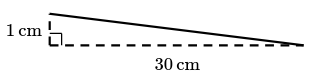
\includegraphics[width=0.4\textwidth]{../images/des_pitagoras_04a.png}
    \end{center}
    \caption{}
    \label{fig:des_pitagoras_04a}
\end{figure}
Cierta tubería debe cubir una distancia horizontal de 700 cm, como se muestra en la figura \ref{des_pitagoras_04b}:
\begin{figure}[H]
    \begin{center}
        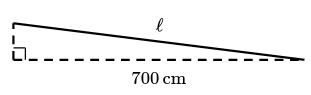
\includegraphics[width=0.4\textwidth]{../images/des_pitagoras_04b.png}
    \end{center}
    \caption{}
    \label{fig:des_pitagoras_04b}
\end{figure}
\textbf{Cuál es la longitud $l$ de esta tubería?}\\
\textit{Redondea tu respuesta a la centésima de metro más cercana.}